% !TEX root = thesis.tex

\section{Results}\label{sec:results}
\subsection{Driving behavior}
Figures~? (from \citet{DeMooij2021}) and~? (from \citet{Kelapanda2021}) show behavioral results.
[Explanation of what we see in their plots.]

\subsection{Pupil size}
\begin{figure}[tp]
  \centering
  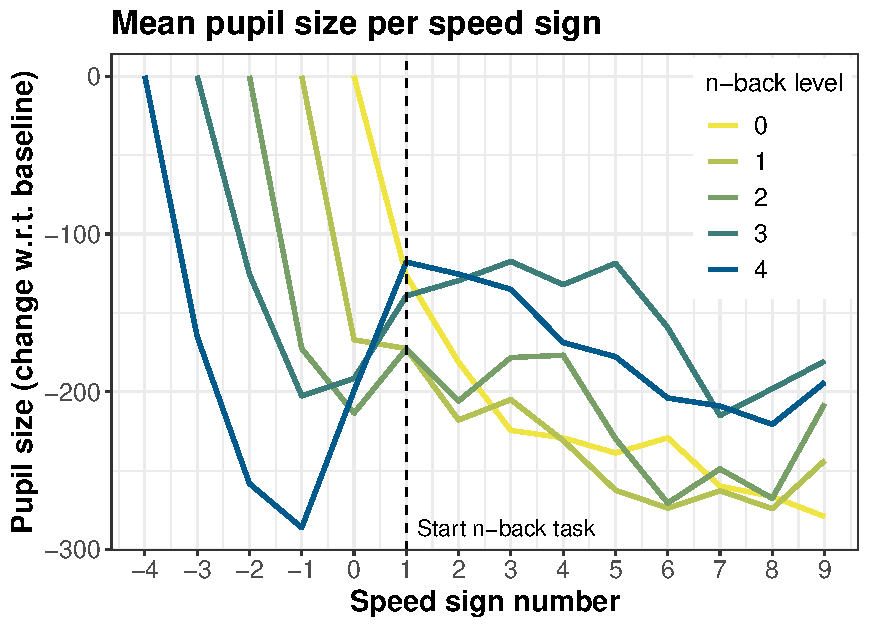
\includegraphics[width=7.5cm]{images/speed_sign_nback.pdf}
  \caption{Mean pupil size over the period between the appearance of two speed signs.
  The dashed vertical line indicates the moment that participants need to start performing the \(n\)-back task by regulating their speed according to the speed signs.
  Pupil size was corrected using subtractive baseline correction and is shown in arbitrary units. 
  The data were smoothed using the loess method.}
  \label{fig:ps-speed-sign}
\end{figure}

Figure~\ref{fig:ps-speed-sign} shows how the pupil size of participants changed within a trial.
There is a visible distinction between change in pupil size for low \(n\)-back levels (\(n = 0,1,2\)) and high \(n\)-back levels (\(n = 3,4\)):
whereas high \(n\)-back levels show a peak in pupil size, low \(n\)-back levels show a decline from the start of the task.
This difference, which can be characterized as an interaction between \(n\)-back level and speed sign number on pupil size, is significant according to an ANOVA with repeated measures [\(F(4,2536)=7.42,\ p < .001\)].
Interestingly, compared to \(n = 3\) the peak in pupil size for \(n = 4\) is higher but shows a sharper decline afterwards.
An explanation for this could be that participants focus their attention on the task at first which causes their pupil to dilate, but then quickly abandon the task because of its difficulty, resulting in a contraction of the pupil.
This theory is supported by the increase in task error for the higher \(n\)-back levels as shown in Figure~?.

\begin{figure}[tp]
  \centering
  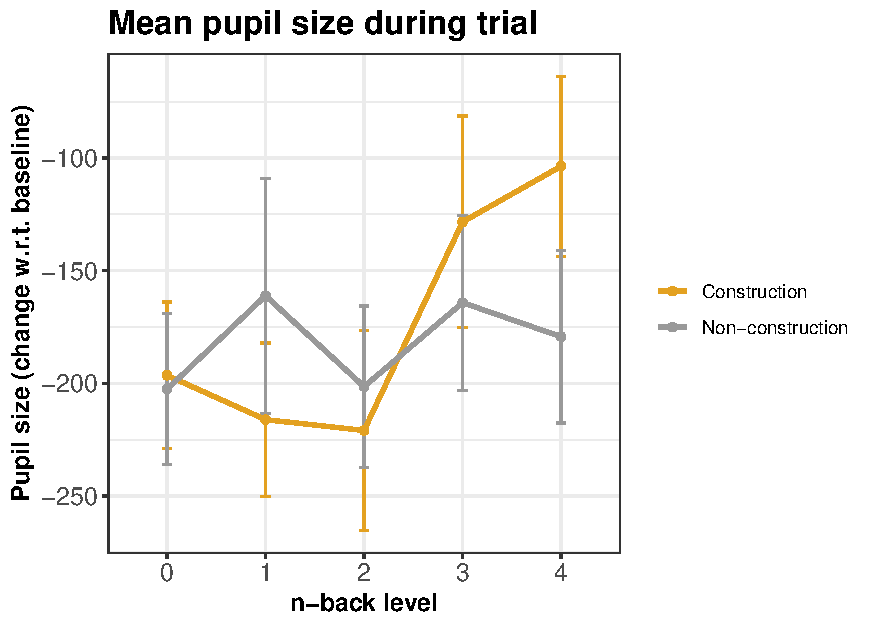
\includegraphics[width=7.5cm]{images/pupil_size_interaction.pdf}
  \caption{Mean pupil size during trial; bars represent standard error.
  Pupil size was corrected using subtractive baseline correction and is shown in arbitrary units.}
  \label{fig:mean-ps}
\end{figure}

Figure~\ref{fig:mean-ps} shows the mean pupil size over an entire trial. 
It suggests that there is no effect of \(n\)-back on pupil size within the non-construction trials.
For the construction trials there seems to be an increase of pupil size by \(n\)-back level more so than for non-construction trials.
However, this suggested interaction between \(n\)-back level and construction on pupil size is not significant [\(F(4,216)=1.50,\ p=.20\)].
Disregarding the difference between construction and non-construction we do find a marginally significant effect of \(n\)-back level on pupil size [\(F(4,221)=2.39,\ p=.052\)].

\subsection{Fixations on speedometer}

\begin{figure}[tp]
  \centering
  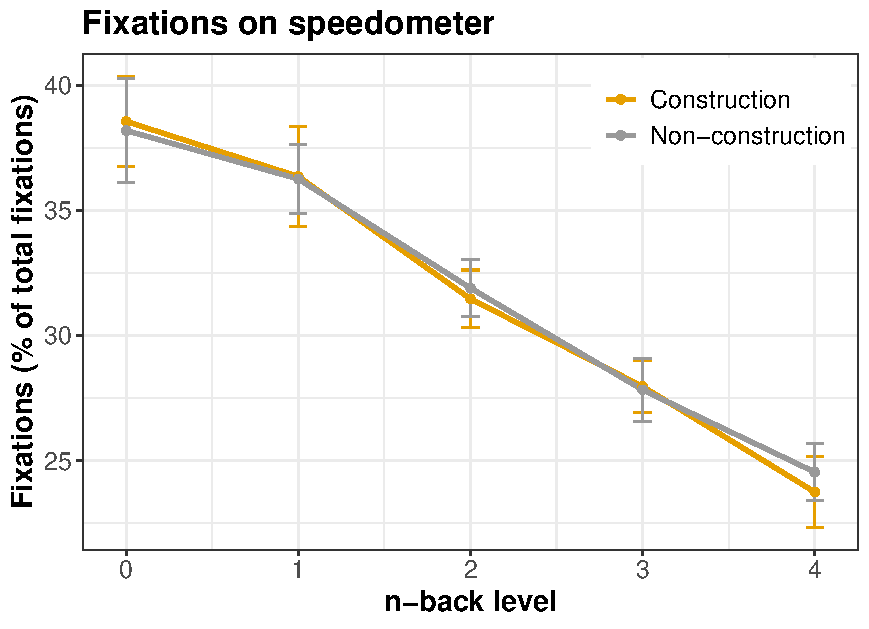
\includegraphics[width=7.5cm]{images/speedometer_interaction.pdf}
  \caption{Number of fixations on the speedometer as a percentage of the total number of fixations for that trial; bars represent standard error.}
  \label{fig:fix-speedometer}
\end{figure}

Figure~\ref{fig:fix-speedometer} shows the number of fixations on the speedometer as a percentage of the total number of fixations for a trial.
Like this figure suggests, there is a significant negative correlation between \(n\)-back level and fixations on the speedometer [\(F(4,221)=84.72,\ p<.001\)] and no effect of construction or an interaction between \(n\)-back and construction. 